\documentclass[3p, 11pt]{elsarticle}


%% Use the option review to obtain double line spacing
%% \documentclass[preprint,review,12pt]{elsarticle}

%% Use the options 1p,twocolumn; 3p; 3p,twocolumn; 5p; or 5p,twocolumn
%% for a journal layout:
%% \documentclass[final,1p,times]{elsarticle}
%% \documentclass[final,1p,times,twocolumn]{elsarticle}
%% \documentclass[final,3p,times]{elsarticle}
%% \documentclass[final,3p,times,twocolumn]{elsarticle}
%% \documentclass[final,5p,times]{elsarticle}
%% \documentclass[final,5p,times,twocolumn]{elsarticle}

%% The graphicx package provides the includegraphics command.
\usepackage[utf8]{inputenc}
\usepackage{graphicx}
\usepackage{hyperref}
\usepackage{amssymb}
\usepackage{amsmath}
\usepackage{amsthm}
\usepackage{subcaption}
\usepackage{siunitx}
\sisetup{group-separator = {,}}

\journal{EJOR}

\usepackage[mathscr]{eucal}
\newcommand{\R}{\mathbb{R}}
\newcommand{\Co}{\mathbb{Co}}
\newcommand{\D}{\mathscr{D}}
\newcommand{\Pp}{\mathscr{P}}
\newcommand{\Cc}{\mathscr{C}}
\newcommand{\E}{\mathscr{E}}
\newcommand{\F}{\mathscr{F}}
\newcommand{\Ww}{\mathscr{W}}
\newcommand{\Rr}{\mathscr{R}}
\newcommand{\norm}[2][2]{\left\lVert#2\right\rVert_{#1}}
\newcommand{\bigO}{\mathscr{O}}
\newtheorem{thm}{Theorem}
\newtheorem{lem}{Lemma}
\newdefinition{rmk}{Remark}
\newdefinition{definition}{Definition}
%\newproof{pf}{Proof}
%\renewcommand\qedsymbol{$\blacksquare$}


\RequirePackage{algorithm, algpseudocode}
\renewcommand{\algorithmicrequire}{\textbf{Input:}}
\renewcommand{\algorithmicensure}{\textbf{Output:}}
\newcommand{\algorithmautorefname}{Algorithm}
\newcommand{\definitionautorefname}{Definition}
\newcommand{\thmautorefname}{Theorem}
\newcommand{\lemmaautorefname}{Lemma}
\newcommand{\lemautorefname}{Lemma}


\begin{document}
	
	\begin{frontmatter}
		
		%% Title, authors and addresses
		
		\title{Algorithms for Planar Maximum Covering Location by Ellipses Problems\tnoteref{t1}}
		\tnotetext[t1]{This paper is the results of the research
			project funded by CAPES.}
		
		%% use the tnoteref command within \title for footnotes;
		%% use the tnotetext command for the associated footnote;
		%% use the fnref command within \author or \address for footnotes;
		%% use the fntext command for the associated footnote;
		%% use the corref command within \author for corresponding author footnotes;
		%% use the cortext command for the associated footnote;
		%% use the ead command for the email address,
		%% and the form \ead[url] for the home page:
		%%
		%% \title{Title\tnoteref{label1}}
		%% \tnotetext[label1]{}
		%% \author{Name\corref{cor1}\fnref{label2}}
		%% \ead{email address}
		%% \ead[url]{home page}
		%% \fntext[label2]{}
		%% \cortext[cor1]{}
		%% \address{Address\fnref{label3}}
		%% \fntext[label3]{}
		
		
		%% use optional labels to link authors explicitly to addresses:
		%% \author[label1,label2]{<author name>}
		%% \address[label1]{<address>}
		%% \address[label2]{<address>}
		
		\author[1]{Danilo Tedeschi}
		\ead{danilo.tedeschi@usp.br}

		
		\author[2]{Marina Andretta}
		\ead{andretta@gmail.com}
					
		%\address{Department of Applied Mathematics and Statistics, Institute of Mathematical and Computer Sciences, University of São Paulo, Avenida Trabalhador São-carlense, 400, Centro, 13566-590, São Carlos, SP, Brazil.}
		%\author{John Smith}
		
		%address{California, United States}
		
		\begin{abstract}
			%% Text of abstract
			Planar Maximum Covering Location by Ellipses is an optimization problem where one wants to place fixed shape ellipses on the plane to cover demand points
			maximizing a function depending on the value of covered points.
			We propose new exact algorithms for two versions of this problem, one where the ellipses have to be parallel to the coordinate axis, and another where they can be freely rotated. 
			Besides finding optimal solutions for previously published instances, including the ones where no optimal solution was known, both algorithms proposed by us were able to obtain optimal solutions for some new larger instances having with up to seven hundred demand points and five ellipses.
		\end{abstract}
		
		\begin{keyword}
			Optimization \sep Covering \sep Combinatorial Optimization
			%% keywords here, in the form: keyword \sep keyword
			
			%% MSC codes here, in the form: \MSC code \sep code
			%% or \MSC[2008] code \sep code (2000 is the default)
			
		\end{keyword}
		
	\end{frontmatter}
	

\section{Introduction}\label{section:introduction}

	
	The Planar Maximum Covering Location Problem (PMCLP) was first introduced in \cite{church:1984}, and can be seen as a category of problems where the coverage of a demand set, a collection of subsets of $\R^2$, is to be maximized by determining the location of facilities in $\R^2$, with coverage being determined by a distance function.
	In \cite{church:1984}, methods for Euclidean and Rectilinear distances versions of the problem were proposed.
	In \cite{drezner, chazelle:1986}, exact algorithms for the Euclidean PMCLP with only one facility are proposed; and in \cite{cabello:2006} an approximation algorithm is proposed for the version with multiple unit disks as facilities.
	A property of the Euclidean PMCLP, which is utilized in the algorithms developed in \cite{drezner, chazelle:1986, cabello:2006}, and in the method proposed in \cite{church:1984}, is that there is an optimal solution which every facility is located in the demand points, or in the intersection of two circles centered at two demand points; we will prove a similar property for ellipses in our work.
	
	It is fair to say that PMCLP with elliptical coverage has not been vastly studied as only two articles have been found on it. In \cite{canbolat}, a mixed-integer non-linear programming method was proposed as a first approach to the problem. For some instances, the method took too long and did not find an optimal solution. Because of that, a heuristic method was developed using a technique called Simulated Annealing, which was able to obtain solutions for the instances proposed in that study.
	The problem was further explored in \cite{andreta}, which introduced the version where the ellipses can be freely rotated, to which an exact and a heuristic method was proposed, and developed a new method for the axis-parallel version of the problem, which was able to obtain optimal solutions for instances that the method proposed by \cite{canbolat} could not.
	The exact method for the version with rotation could not obtain optimal solutions within a predefined time limit for several instances, the heuristic method though returned solutions for every instance, and impressively enough, obtained optimal solutions for every verifiable instance.
	
	We study two versions of PMCLP with elliptical coverage facilities in this work. For both of them, each ellipse is defined to have a fixed shape and an undefined location, which is part of the solution.
	In the first version, introduced in \cite{canbolat}, all the ellipses are restricted to be axis-parallel, while in the second version, introduced in \cite{andreta}, this constraint is dropped, and all the ellipses can be freely rotated.
	The first version will be referred to as Planar Maximum Covering Location by Ellipses Problem (MCE) and the second one as  Planar Maximum Covering Location by Ellipses with Rotation Problem (MCER).
	
	\section{Problem Definition}
	
	An instance of MCE and MCER is given by $n$ demand points $\Pp=\{p_1, \dots, p_n\}$, $p_j\in\R^2$; $n$ weights $\Ww=\{w_1, \dots, w_n\}$, with $w_j\in\R$, $w_j>0$ being the weight of the $j$-th point; and $m$ shape parameters $\Rr=\{(a_1, b_1), \dots, (a_m, b_m)\}$, with $(a_j, b_j)$ being the semi-major and semi-minor of the $j$-th ellipse, with $a_j > b_j$. We define a list of functions $\E=\{E_1, \dots, E_m\}$ representing the coverage area of each facility. For MCE $E_j\colon\R^2\to\R^2$ is defined as
	\begin{equation}
	E_j(q) = \{p \in \R^2 \colon (p_x-q_x)^2/a_j^2 + (p_y-q_y)^2/b_j^2 \le 1\}.
	\end{equation}
	For MCER, we define $E_j \colon \R^2 \to \R^2 \times [0, \pi)$ as
	\begin{equation}
		E_j(q, \theta) = \left\{p \in \R^2 \colon 
		\left|\left|
		\left(
		\begin{array}{rr}
		\cos{\theta}/a_j & \sin{\theta}/a_j\\
		\sin{\theta}/b_j & -\cos{\theta}/b_j
		\end{array}
		\right)
		\left(
		\begin{array}{c}
		p_x-q_x\\
		p_y-q_y
		\end{array}
		\right)
		\right|\right|_2
		\le 1
		\right\}.
	\end{equation}
	
Let $w : A \subset \Pp \to \R$ be a function which takes a subset of the demand set and returns the sum of the weights of the points in $A$. Then, we define MCE as the optimization problem 
\begin{equation}
\max_{q_1, \dots, q_m} \sum_{j=1}^m w(\Pp \cap E_j(q_j)),
\end{equation}
and similarly MCER as
\begin{equation}
\max_{(q_1, \theta_1), \dots, (q_m, \theta_m)} \sum_{j=1}^m w(\Pp \cap E_j(q_j, \theta_j)).
\end{equation}

To make the notation more clear, we denote an instance of MCE or MCER as the tuple $(\Pp, \Ww, \Rr)$, and a solution of MCE as $Q:=(q_1, \dots, q_m)$, and a solution of MCER as $Q:=((q_1, \theta_1); \dots; (q_m, \theta_m))$. We also use $\partial$ as the boundary operator, for example, $\partial E_1(q_1)$ denotes an ellipse with shape parameters $(a_1, b_1)$ centered at $q_1$ given an instance of MCE.

\section{An algorithm for MCE}\label{section:mce}

Similarly to the method developed in \cite{church:1984} for the Euclidean PMCLP, we will describe a Candidate List Set (CLS) of possible locations for each ellipse and then propose an algorithm that constructs solutions combining the possible locations in each ellipse's CLS.
Also, based on the approach of \cite{church:1984} for the Euclidean PMCLP, and in \cite{chazelle:1986} for the problem of covering points by one unit disk, we will construct the CLS for each ellipse by using a property of the one-facility MCE.
Although, it is intuitive that it is possible to adapt the ideas used for solving the problems involving Euclidean disks for axis-parallel ellipses, using the results of \cite{bi}, which studies the problem of determining the intersection of $n$ strictly convex disks with fixed radius, we will prove that for MCE, we have all the necessary geometric properties to develop an algorithm following those approaches.

We start by introducing a lemma stating that any solution of the one-facility MCE can be related to the intersection of coverage regions of ellipses centered at the points covered in that solution. 

\begin{lem}\label{lema:mce-mwc}
	Let $(\Pp, \Ww, \{(a, b)\})$ be an instance of MCE, and $q\in \R^2$. If $\Pp \cap E(q) = A$, then $q \in \cap_{p\in A} E(p)$.
\end{lem}
\begin{proof}
	Let $u, v \in \R^2$, then we have that $u \in E(v)$ if, and only if $v \in E(u)$, which is proved simply by observing that:
	\begin{equation}\label{eq:peq}
	u \in E(v) \Leftrightarrow ||u-v||_{a, b, 0} \le 1 \Leftrightarrow v \in E(u).
	\end{equation}
	As $\Pp \cap E(q) = A$ can be written as: for all $p \in A$, $p \in E(q)$. Then, using \autoref{eq:peq}, we get that for all $p \in A$, $q \in E(p)$, which implies that $q \in \cap_{p\in A} E(p)$.
\end{proof}



%To define this equivalent problem, we need to first state an ellipse's property.
%Let $(\Pp, \Ww, \{(a, b)\})$ be an instance of MCE with one facility, and  $p, q \in \R^2$, we have that

%The equivalent problem is given by $n$ ellipses with shape parameters $(a, b)$ centered at $\Pp$. Let $q\in\R^2$ be a solution of MCE for one facility, by applying \autoref{eq:peq} to every point covered by $E(q)$, we obtain that
%\begin{equation}\label{eq:mce-mwc}
%\Pp \cap E(q) = \{p_i\in\Pp \colon q\in E(p_i)\},
%\end{equation}
%which implies that the problem of determining $q\in\R^2$ to maximize $w(\{p_i\in\Pp \colon q\in E(p_i)\})$, is equivalent to MCE for one facility. This changes the problem from determining a location for an ellipse given $n$ points to the problem of finding a point given $n$ ellipses with fixed locations.

%Let $A\subset \Pp$, from \autoref{eq:mce-mwc}, we have that if $\Pp \cap E(q) = A$ then $q \in \cap_{p\in A} E(p)$. 

From , if we could identify every 

Let $A \subset \Pp$, $|A|>1$, let us consider the intersection region $\cap_{p\in A} E(p) \neq \emptyset$. From \autoref{lema:mce-mwc}, we can also conclude that if $q \in \cap_{p\in A} E(p)$, then $A \subset \Pp \cap E(q)$.


In \cite{church:1984}, for the Euclidean PMCLP, it was proved that the border of this region contains at least one point that is an intersection between two fixed-radius circles with centers in $A$. This, as it turns out, is also true for ellipses, and a proof can be obtained from \cite{bi} where the problem of determining the intersection region of $n$ fixed-radius disks in a strictly convex normed plane is studied.
From that, we can conclude that there exists $u, v \in A$ and $q \in \partial E(u) \cap \partial E(v)$, such that $q \in \cap_{p\in A} E(p)$.
Before defining the CLS for each ellipse, we introduce a lemma stating two basic, and yet important properties about the intersection between two axis-parallel ellipses that have the same shape and distinct locations.

\begin{lem}\label{lema:e2p}
	Let $E$ be the coverage region of an axis-parallel ellipse with shape parameters $(a,b)$; and $v \in \R^2$, $v\neq0$. Then $|\partial E(0) \cap \partial E(v)| \le 2$, and $\partial E(0) \cap \partial E(v)$ can be determined analytically.
\end{lem}

\begin{proof}
	To determine the intersection points, consider the equality between the equations of $\partial E(0)$ and $\partial E(v)$:
	$x^2/a^2 + y^2/b^2 = (x-v_x)^2/a^2 + (y-v_y)^2/b^2.$
	This expression can be reduced to $y=\alpha x + \beta$, for some $\alpha, \beta$, which can then be plugged into $\partial E(0)$'s equation obtaining $x^2/a^2 + (\alpha x + \beta)^2/b^2 = 1$.
	We obtain the intersection points by solving this quadratic equation for $x$, and then, for each value of $x$,  determining $y$ from $y=\alpha x + \beta$.
\end{proof}
Next, we define the CLS of each ellipse, considering also the case where, in an optimal solution, an ellipse covers only one point.
\begin{definition}\label{def:cls_mce}
	Given an instance of MCE, for all $k \in \{1, \dots, m\}$, we define the CLS for the $k$-th ellipse as
	\begin{equation}
	S_k = \Pp \cup \left(\bigcup_{1 \le i < j \le n} \partial E_k(p_i) \cap \partial E_k(p_j) \right).
	\end{equation}
\end{definition}

By \autoref{lema:e2p}, the CLS for each ellipse can be computed in $\bigO(n^2)$, and $|S_k| \le n + 2\binom{n}{2}$. Next, we establish a lemma stating that the set of solutions obtained by combining the possible locations in each ellipse's CLS contains at least one optimal solution.

\begin{thm}\label{thm:mce}
	Given an instance of MCE, and $S_1, \dots, S_m$ as defined by \autoref{def:cls_mce}, then the set $\Omega = \{(q_1, \dots, q_m) \colon \textnormal{ for all }q_k \in S_k \}$ contains an optimal solution of MCE and $|\Omega| \le n^{2m}$. 
\end{thm}
\begin{proof}
	Let $Q^*$ be an optimal solution of MCE for the given instance. Then, we are going to prove that there exists $Q' \in \Omega$, which is also optimal.
	
	For each $k=1, \dots, m$, let $X_k = \{p_i \in \Pp\colon p_i \in E_k(q_k^*)\}$.
	
	%If $|X_k| = 0$, then any $q_k \in S_k$ makes $X_k \subset \Pp \cap E_k(q_k)$.
	
	If $|X_k| \le 1$, then there is at least one element in $S_k$ that makes $X_k \subset \Pp \cap E_k(q_k)$.
	
	If $|X_k| > 1$, then let $Y_k = \cap_{p \in X_k}E_k(p)$. By the results of \cite{bi}, we have that the boundary of $Y_k$ has vertices in the pairwise intersections of $\{\partial E_k(p) \colon p \in X_k\}$. Therefore, at least one vertex of $Y_k$ is in $S_k$, and any of those vertices produce a solution that covers at least the same points covered by $Q^*$.
	
	Lastly, we have that $|S_k| \le 2\binom{n}{2} + n = n(n+1)/2 \le n^2$. Hence, $|\Omega| \le n^{2m}$.
\end{proof}

With all this in hand, we define \autoref{algoritmo:mce}, which goes through every possible combination in the CLS of each ellipse. As evaluating each solution can be done in $\bigO(nm)$, we have that \autoref{algoritmo:mce} has $\bigO(mn^{2m+1})$ runtime complexity. 
In \autoref{section:numerical}, we give more details about the implementation of \autoref{algoritmo:mce} and analyze some numerical experiments for instances proposed in \cite{canbolat, andreta}, and for some new ones.

\begin{algorithm}
	\caption{Algorithm for MCE}\label{algoritmo:mce}
	
	\begin{algorithmic}[1]
		\Require{A set of points $\Pp=\{p_1,\dots,p_n\}$, a list of weights $\Ww=\{w_1, \dots, w_n\}$, and a list of shape parameters $\Rr=\{(a_1, b_1), \dots, (a_m, b_m)\}$.}
		
		\Ensure{An optimal solution for MCE.}
		
		\item[]
		\Procedure{$MCE$}{$\Pp, \Ww, \Rr$}
		\State \Return $MCE_{bt}(\Pp, \Ww, \Rr, 1)$
		\EndProcedure
		\State
		\Procedure{$MCE_{bt}$}{$Z, \Ww, \Rr, j$}
		\If{$j = |\Rr|+1$}
		\State \Return $0$
		\EndIf
		
		\State $(q_j^*, \dots, q_m^*) \gets (0, \dots, 0)$
		\State Let $S_j$ be the CLS for the $j$-th ellipse as defined by \autoref{def:cls_mce}.
		%\State $S_j \gets \textnormal{CLS-MCE}(Z, a_j, b_j)$
		\For{$q_j \in S_j$}
		\State $Cov \gets \Pp \cap E_j(q_j)$
		\State $(q_{j+1}, \dots, q_m) \gets MCE_{bt}(Z \setminus Cov, \Ww, \Rr, j+1)\}$
		
		\If{$w(\cup_{k=j}^m Z \cap E_k(q_k)) >  w(\cup_{k=j}^m Z \cap E_k(q_k^*))$}
		\State $(q_j^*, \dots, q_m^*) \gets(q_j, \dots, q_m)$
		\EndIf
		\EndFor
		
		\State \Return $(q_j^*, \dots, q_m^*)$
		\EndProcedure
	\end{algorithmic}
\end{algorithm}

\section{Determining every location of an ellipse given its shape and three points}\label{section:e3p}
	
The problem of finding every center and angle of rotation of a fixed shape ellipse which makes it have three points on its border is presented in this section. Even though its simple statement--it is short and uses only basic mathematical concepts--we were not able to find any work on it, or even on related problems. 
As a result, starting from scratch, we ended up trying a handful of approaches with most of them failing on the way. We try to give a review of some of those, and also make a case for the method we propose in terms of velocity of convergence and quality of the solutions that it finds.

We refer to this problem as \sigla{E3PNT}{Ellipse by Three points}, and an instance of it is given by three points $u, v, w \in \R^2$ and $E$, an ellipse with shape parameters $(a, b) \in \R^2_{>0}$, with $a > b$. A solution of E3PNT is a pair $(q, \theta) \in \R^2\times[0, \pi]$, such that $\{u, v, w\} \subset \tilde{E}(q, \theta)$. In other words, the goal is to develop a method to find every solution of E3PNT. 


\section{Transforming the problem}

To make it simpler, let us translate the system, so the point $u$ is at $(0,0)$. Then, we assume that the ellipse is actually axis-parallel and the points are the ones rotating. When an angle is found such that the three points lie on the border of the axis-parallel ellipse, a linear transformation can be applied to compress the x-axis by $\frac{b}{a}$, transforming the ellipse into a circle of radius $b$. This transformation can be seen on \autoref{fig:circumscribed-circle} where a solution of the E3PNT is transformed into a solution of the problem of finding a circumscribed circle of a triangle. 
This process can be parametrized by the angle of rotation of the points, as described by \autoref{eq:trpnts}, and because of the invertibility of linear transformations solutions for E3PNT can be obtained by reversing the transformations.

\begin{figure}
	\centering
	\caption{Transforming an ellipse into a circle. T1, T2, and T3 represent the steps of the transformation.}
	\includegraphics{tex/figures/scripts/circumscribed-circle}
	\fautor
	\label{fig:circumscribed-circle}
\end{figure}
\begin{equation}\label{eq:trpnts}
\varphi(p, \theta)=\left[\begin{array}{cc}
\frac{b}{a}&0\\
0&1
\end{array}\right]
\left[\begin{array}{cc}
\cos{\theta}&\sin{\theta}\\
-\sin{\theta}&\cos{\theta}
\end{array}\right]\left[\begin{array}{c}
p_x\\
p_y
\end{array}\right].
\end{equation}

Then, the problem to be solved is finding a circumscribed circle of the triangle formed by the points $(0, 0), \varphi(v, \theta)$ and $\varphi(w, \theta)$, such that the circle has radius $b$. As, for three non-colinear fixed points, there is always an unique circumscribed circle for the triangle formed by those three points, the only variable to be determined ends up being the angle of rotation $\theta$.

Let $A(\theta)$ be the area of the triangle formed by the points $(0, 0), \varphi(v, \theta)$ and $\varphi(w, \theta)$--note that the transformation does not preserve distance or area. Then, the radius $R$ of the circumscribed circle is given by \autoref{eq:circumscribed_circle} \cite[p.~189]{johnson1960}.

\begin{equation}\label{eq:circumscribed_circle}
R = \dfrac{\norm{\varphi(v, \theta)}\norm{\varphi(w, \theta)}\norm{\varphi(v, \theta)-\varphi(w, \theta)}   }{4A(\theta)}.
\end{equation}

Imposing the radius to be equal $b$ and squaring to eliminate the square roots present in the Euclidean distance, a function $\xi : [0, \pi) \mapsto \mathbb{R}_{>0}$ is defined by \autoref{eq:circumscribed_circle_b} in such a way that its zeros determine solutions to the E3PNT's instance. Two questions about $\xi(\theta)$ that arise are: is its set of roots finite? And, can they be found analytically?

\begin{equation}\label{eq:circumscribed_circle_b}
\xi(\theta) = 16b^2A(\theta)^2 - \norm{\varphi(v, \theta)}^2\norm{\varphi(w, \theta)}^2\norm{\varphi(v, \theta)-\varphi(w, \theta)}^2.
\end{equation}

\subsection{The number of solutions is limited}

The method developed on \autoref{chapter:ellipses_n} iterates over every solution of E3PNT for every triplet of points, this is only possible if the size of this set of solutions is limited. Also, if this was not true, it would be very difficult to describe a method to get every solution which could be infinite.

It turns out that $\xi$ can be written as a real trigonometric polynomial of degree $6$ in the format given by \autoref{eq:trig_poly_2}, which implies that it can have up to $12$ distinct roots.
 To show that, just note that it is possible to write $\norm{\varphi(v, \theta)}^2$ and $A(\theta)^2$ in that form, as it can be seen on \autoref{eq:dd} and \autoref{eq:dd2}. It is also possible to see that the term of higher the degree of $\xi$ is the multiplication of the three squared distances. As $\norm{\varphi(v, \theta)}^2$ has degree $2$, the degree of $\xi$ is $6$.
\begin{align}\label{eq:dd}
	\norm{\varphi(v, \theta)}^2 = (v_x\frac{b}{a}\cos\theta + v_y\frac{b}{a}\sin\theta)^2 + (v_y\cos\theta - v_x\sin\theta)^2\\
	\label{eq:dd2} A(\theta)^2=\dfrac{1}{4}\det\left(
	\begin{array}{cc}
		v_x\frac{b}{a}\cos\theta + v_y\frac{b}{a}\sin\theta&v_y\cos\theta - v_x\sin\theta\\
		w_x\frac{b}{a}\cos\theta + w_y\frac{b}{a}\sin\theta&w_y\cos\theta - w_x\sin\theta
	\end{array}\right)^2
\end{align}

Because ellipses are symmetrical with respect to their major-axis, and any rotation in the interval $[0, \pi)$ is identical to a rotation in $[\pi, 2\pi)$, the number of different solutions is cut in half.
Therefore, the number of angles of rotation and centers that an ellipse of fixed shape can be placed, so it has three fixed points on its border is limited to $6$.

\section{An attempt using the conic general equation}

The idea of this approach was to use the six-parameter conic equation to represent an ellipse. This equation is given by \autoref{eq:gen_ellipse}.

\begin{equation}\label{eq:gen_ellipse}
Ax^2+Bxy+Cy^2+Dy+Ex+F=0.
\end{equation}
This equation actually represents any conic, for it to be an ellipse the condition $B^2 -4AC < 0$ must be satisfied.

Setting the first point to be the origin, we get $F=0$, using the other two points, it is possible to write $D$ and $E$ in terms of $A, B, C$. As any multiple of \autoref{eq:gen_ellipse} represents the same conic, we can set $B$ to be equal $1$. Then, we end up with two variables, $A$ and $C$, and still need to impose that the final equation represents an ellipse and its major-axis and minor-axis have the predefined value. Let $\Delta=4AC-B^2=4AC-1$, \autoref{eq:gen_ellipse_a} and \autoref{eq:gen_ellipse_b} for both major-axis and minor-axis respectively, assuming $F=0$.

\begin{align}\label{eq:gen_ellipse_a}
a^2 = \dfrac{2\dfrac{AE^2 -BDE +CD^2}{\Delta}}{A + C - \sqrt{1 + (A-C)^2}}\\
\label{eq:gen_ellipse_b}b^2 = \frac{2\dfrac{AE^2 -BDE +CD^2}{\Delta}}{A + C + \sqrt{1 + (A-C)^2}}
\end{align}

These two equations define two curves in $\R^2$ with $A$ and $C$ being the chosen variables. The solutions lie in the set of intersection of these curves. Finding this set was judged to be non-trivial and probably could be approximated numerically, however, we decided not to further pursue this approach.

Another idea which has been explored was working with the ratio $\frac{a^2}{b^2}$ which becomes an expression that allows $A$ to be written as a function of $C$. This function appeared, at first we thought, to be monotonic, we tried to develop a method based on that, however, cases where the function does not behave as nicely were found. It is likely that developing a method to approximate solutions working with this function is possible, but we decided not to continue on this track.


\section{An approximation method}

One of the most useful techniques when dealing with complicated functions is approximation. They appear in various methods whenever a derivative or integral needs to be calculated or for example, in our case, when the roots of a function need to be determined. In general, one has a function $f$ that is part of a family of functions $\mathcal{A}$ and wants to select a simpler function $f^*$ from a set of functions $\mathcal{A^*}$, such that $f^*$ is close enough to $f$ \cite[p.~3]{powell}. For this problem, the approximation of $\xi(\theta)$ on the interval $[0, \pi)$ is considered. The approximation set of functions is going to be the set of $n$-degree Chebyshev polynomials which the roots can be found through determining the eigenvalues of a $n$ by $n$ matrix.


\subsection{Chebyshev interpolation}

Chebyshev polynomials are widely used in Numerical Analysis in areas like numerical integration, polynomial approximation, and ordinary and partial differential equations.
They are also very useful in practice and are present in extension libraries in Python and MATLAB.

Because of the scope of this work, only a brief introduction of Chebyshev polynomials of the first kind and its usage in polynomial interpolation is given. For a more thorough work on the subject, please check the book by \citeonline{chebbook}.

We refer to $T_n : [-1, 1] \mapsto [-1, 1]$ as the $n$-degree Chebyshev polynomial of the first kind, and it is defined as follows:

\begin{equation}
T_n(x) = \cos({n\arccos x})
\end{equation}

It is important to mention that this definition can be extended to the whole real line. Using some trigonometric identities, $T_n$ can also be expressed as a recurrence relation:

\begin{equation}
T_n(x) = 2xT_{n-1}(x) - T_{n-2}(x).
\end{equation}

An important property worth bringing up is that Chebyshev polynomials are orthogonal and form a basis for the polynomial space. This implies that any $p_n$ of degree up to $n$ can be expressed as a truncated Chebyshev series:

\begin{equation}\label{eq:chebseries}
p_n(x) = \sum_{j=0}^{n} a_j T_j(x).
\end{equation}

One of the greatest qualities of Chebyshev polynomials is its numerical stability. \citeonline{gautschi:1979} showed that the matrix that maps polynomials onto its coefficients written in the power form\footnote{A polynomial is in the power form or the monomial form if it can be written as $\sum_{j=0}^{n}a_jx^j$} has a condition number that grows exponentially with $n$. On the other hand, the matrix that converts polynomials to the Chebyshev basis as \autoref{eq:chebseries}, has a linear condition number bounded by $\sqrt{2}n$.

Polynomial interpolation is a form of approximating a function by a polynomial of degree $n$ that passes through $n+1$ chosen points. In fact, this polynomial is unique and it is determined by Lagrange's formula:

\begin{equation}\label{eq:lagrange}
f_n(x) = \sum_{j=0}^{n} f(x_j)\dfrac{\prod_{k \neq j}^{n+1} (x-x_k)}{\prod_{k \neq j}^{n+1} (x_j-x_k)},
\end{equation} 
with $f$ being the function to be approximated, and $f_n$ the unique $n$-degree polynomial that passes through $\{(x_j, f(x_j)): j=0, 1, \dots n\}$. Because of the uniqueness of interpolant polynomials, there is a direct link between the quality of an approximation and the points chosen to interpolate. As a matter of fact, depending on the points one chooses, even increasing the degree of the interpolation makes the approximation worsen. This is known as Runge's phenomenon and an example can be seen in \citeonline[p.~37]{powell} where uniformly spaced points are chosen to interpolate the function $f(x) = (1+x^2)^{-1}$ on the interval $[-5, 5]$. 

That is where Chebyshev interpolation comes in. Instead of choosing $n+1$ arbitrary points, the $n+1$ roots of $T_{n+1}$, which are also known as Chebyshev Nodes, are chosen as the interpolation points:
\begin{equation}
x_j = \cos{\left(\dfrac{\pi(k-\frac{1}{2})}{n+1}\right)},
\end{equation}
for $j=1, \dots, n+1$. This particular choice defeats Runge's phenomenon and provides a convergent approximation. 

Note that, if the domain of the function to be interpolated is defined on a range other than $[-1, 1]$, let us say $[a, b]$, then a transformation can be done to map it to the Chebyshev Nodes' domain:
\begin{equation}
\hat{x_j} = \frac{a+b}{2} + \frac{b-a}{2}x_j.
\end{equation}

Then, the Chebyshev interpolation of a function $f: [a, b] \mapsto \R$ can be determined using Lagrange's formula and the points $\hat{x}_1, \dots, \hat{x}_n$. 
As it was mentioned, finding the roots of a polynomial written in the monomial form can be done by determining the eigenvalues of a so-called Frobenius companion matrix. For small $n$ this works fine, however, converting the polynomial obtained by \autoref{eq:lagrange} to the power form, as $n$ grows, becomes a very ill-conditioned problem. 
An alternative method can be found in \citeonline{boyd:2013} where the Chebyshev interpolation is calculated directly as a truncated Chebyshev series, as in \autoref{eq:chebseries}, in $\bigO(n^2)$. Also, given a polynomial written in the Chebyshev basis, a $n\times n$ matrix can be constructed, such that its eigenvalues are the roots of that polynomial. \citeonline{boyd:2013} refers to this matrix as the Chebyshev-Frobenius companion matrix.

Therefore, the whole process of interpolating and finding the roots can be done using only Chebyshev polynomials, which have great numerical stability. Also, Chebyshev-Frobenius matrices have the same property as companion matrices which allows their eigenvalues to be found by a QR decomposition. Summing the two steps, a $\bigO(n^2)$ algorithm can be achieved.

The last question that needs to be addressed is how close the roots of the Chebyshev interpolant $f_n$ are to the roots of $\xi$?

Even though $\xi$ is complicated enough, in a sense that finding its roots directly is no trivial task, it is a very well-behaved function: it is analytic and  has infinitely many continuous and integrable derivatives. This satisfy all the requirements of the result in \citeonline[p.~28]{gottlieb} which says that if a function has $m$ continuous and integrable derivatives on a closed interval, then its absolute difference between the Chebyshev truncate series is $\bigO(n^{-m})$. Also, in \citeonline{battles:2004} a theorem is presented stating that if a function is analytic on a neighborhood of $[-1, 1]$, then the convergence is $\bigO(C^n)$, for some $C<1$.

To choose the degree of the interpolation we use the last coefficient rule-of-thumb introduced by \citeonline[p.~50]{boyd:2001}. There is no guarantee that this method will choose $n$, such that $f_n$ is close enough to $\xi$ everywhere on $[0, \pi)$, nonetheless, in practice, it is taken to be a good estimate for the error $r_n$:
\begin{equation}
r_n = \max_{0 \le \theta \le \pi} |f_n(\theta) - \xi(\theta)|.
\end{equation}


\section{Converting $\xi$ into a polynomial}

On \autoref{chapter:definitions} a brief introduction is given on how to get the roots of a polynomial. For that reason, we discuss two ways of converting $\xi$ into a polynomial in this section. Symbolic computing was used to compute the polynomials, in practice an external Python library called SymPy was utilized (see \citeonline{sympy} for more details).

The first attempt was using the identity $x = \tan{\frac{\theta}{2}}$ from which it is possible to construct a $12$-degree polynomial. At first,  the root-finding algorithm described on \autoref{chapter:definitions} seemed to work fine and return every solution of E3PNT, however, we later found out that for some instances, priorly known roots were not being found. The cause was not for sure identified, but a good guess would be that for angles which are greater than $\frac{\pi}{4}$, $x$ starts growing too rapidly which could lead to numerical instability.

The second approach is based on a idea published on \citeonline{boyd:2006} which uses the identities on \autoref{eq:complex_trig} to convert real trigonometric polynomials into univariate complex polynomials in order to obtain its roots using the companion matrix scheme.
Also, in \citeonline{weidner} it is said that computing the roots of a real trigonometric polynomial through this transformation does not yield loss of accuracy.

\begin{align}\label{eq:complex_trig}
\cos{\theta} = \dfrac{e^{i\theta} + e^{-i\theta}}{2}\\
\sin{\theta} = \dfrac{e^{i\theta} - e^{-i\theta}}{2i}.
\end{align}

It is possible to show that with that substitution and changing the variable to $z=e^{i\theta}$, we obtain the following function $g : \mathbb{S} \mapsto \mathbb{C}$, with $\mathbb{S}$ being the unit circle ($\mathbb{S} = \{z \in \mathbb{C} : |z|=1\}$):

\begin{equation}
g(z)=\sum_{k=0}^{12} c_k z^{k-6},
\end{equation}
for some $c_0, \dots, c_{12} \in \mathbb{C}$. Even though $g$ is not a polynomial, it is easy to obtain one from it. Firstly, the negative exponentials need to be shifted, this can be done by just multiplying $g$ by $z^6$. Secondly, the domain cannot be restricted to the unit circle, so we define $h : \mathbb{C} \mapsto \mathbb{C}$ as:
\begin{equation}
h(z) = z^6 g(z) = \sum_{k=0}^{12} c_k z^k.
\end{equation}

Then, by its definition is possible to see that every root of $g$ is also a root of $h$. Conversely, every root $\hat{z}$ of $h$ which is in $\mathbb{S}$--or $|\hat{z}|=1$--is also a root of $g$. Naturally, the angle of a root $\hat{z}$ of $g$ is a root of $\xi$ by Euler's Formula.

It is possible to make another reduction to obtain a degree-$6$ polynomial from $h$ whose roots form a superset of the roots of $g$. As it has been mentioned on this chapter, an ellipse is symmetric with respect to its own axis. This means $\theta$ and $\pi + \theta$ are equivalent angles of rotation for any ellipse, thus $\xi(\theta) = \xi(\pi + \theta)$\footnote{$\xi$ is only defined over $[0, \pi)$, so this equality is not actually valid.}. 
On \autoref{chapter:definitions}, it was stated that the angle of $z$ and $-z$ has the same symmetry with each other as an ellipse's angle of rotation:
\begin{equation*}
angle(-z) = \pi + angle(z).
\end{equation*}
From that, as $g(e^{i\theta})=\xi(\theta)$ for every $\theta \in [0, 2\pi)$, we conclude that $g(-z)=g(z)$. This implies that $h$ is, in fact an even polynomial, or that $h(-z) = h(z)$ is true for every $z\in\mathbb{C}$:
\begin{align}
h(-z) = (-z)^6g(-z) = z^6g(z).
\end{align}
Therefore, all the odd degree coefficients of $h$ are $0$ and we can define the $6$-degree polynomial $f : \mathbb{C} \mapsto \mathbb{C}$ with the substitution $y=z^2$:
\begin{equation}
f(y) = \sum_{k=0}^{6} c_{2k} y^k.
\end{equation}
Then from every root $\hat{y}$ of $f$, two roots of $h$ can be obtained: $\sqrt{\hat{y}}$ and $-\sqrt{\hat{y}}$. As the angle of $-\sqrt{\hat{y}}$ is not between $[0, pi)$ we can ignore it. Note that the the square root of $\hat{y}$ does not need to be calculated, as only the angles are needed and they can be obtained by:
\begin{equation}
angle(\sqrt{z}) = angle(z)/2.
\end{equation}
Finally, using the QR algorithm mentioned on \autoref{chapter:definitions} a $\bigO(n^3)$ algorithm, with $n=6$, can be constructed for E3P.

It is also worth mentioning that a pattern on the coefficients of $f$ was identified, and maybe for future work it can be used for further improvements. Analyzing the polynomials produced for several instances, the following seems to true:
\begin{equation}
c_k = \hat{c_{6-k}},
\end{equation}
for $k=0, \dots, 6$. For now, we do not have any ideas on how it could be proved. Nevertheless, this seems to lead somewhere interesting because this condition guarantees that $f$ is a self-reciprocal polynomial which implies that its roots will always come in pairs $(\hat{z}, 1/\hat{z})$.

\section{Numerical Experiments}

In this section we run some experiments to verify how big the interpolation degree must be for a good precision to be achieved. 
Let $f_n$ be the $n$-degree Chebyshev interpolation of $\xi$, we define the interpolation error $r_n$ as:



Then, we want to determine the smallest $n$, such that $r_n \le \epsilon$, for a predefined $\epsilon$. Unfortunately, calculating $r_n$ involves taking samples from both functions on the whole interval, which is not viable computationally. In \citeonline[p.~50]{boyd:2001} a rule-thumb for estimating the interpolation error is given. It is worth mentioning that this rule 

It uses a theorem that states that $r_n$ is limited by the sum of the coefficients of the Chebyshev series that were removed by the truncation. The rule-of-thumb for estimating $r_n$ is given by:

\begin{equation}
r_n \approx |a_n|.
\end{equation}

Note that 

Obtaining an expression for it is not trivial, and sampling the whole interval is not viable computationally. 

Therefore, an estimation of $r_n$ is used to measure how good is the approximation.

Also we adopt two suggestions from \cite{boyd:2013}. The first is to divide the interval into $K$ subintervals to achieve a precision without having to increase the degree of the interpolant too much. The second is to use a couple of Newton's iterations to refine the roots found. 

Let $\theta^*$ be a root of $f_n$, then we measure the error associated with that root as $|\xi(\theta^*)|$. For the numerical experiments, we considered every triplet of points from an instance with $25$ points. Then for some values of $K$ and $n$ we define the error as the maximum error for every root that were found.

\begin{figure}
	\centering
	\caption{The interpolation error measured on roots that were found.}
	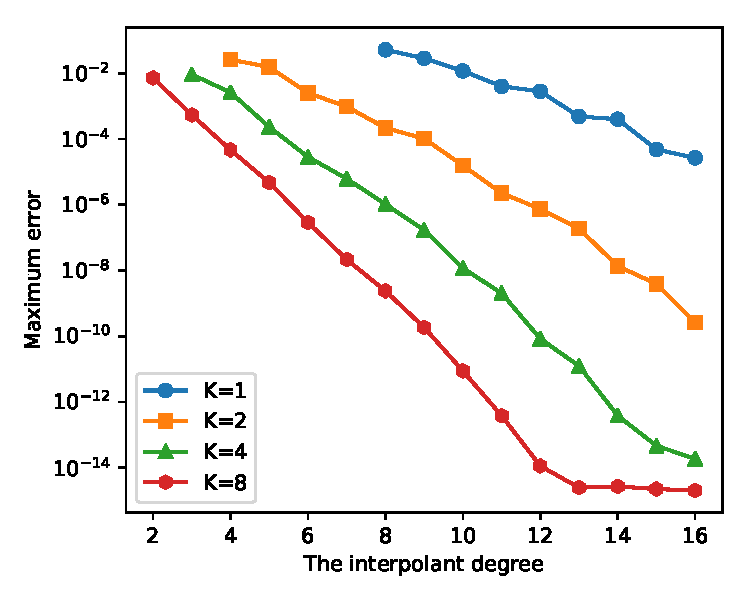
\includegraphics{tex/figures/interpolant_error}
	\fautor
	\label{fig:interpolant_error}
\end{figure}

\begin{figure}
	\centering
	\caption{The interpolation error measured on roots that were found after three Newton's iterations.}
	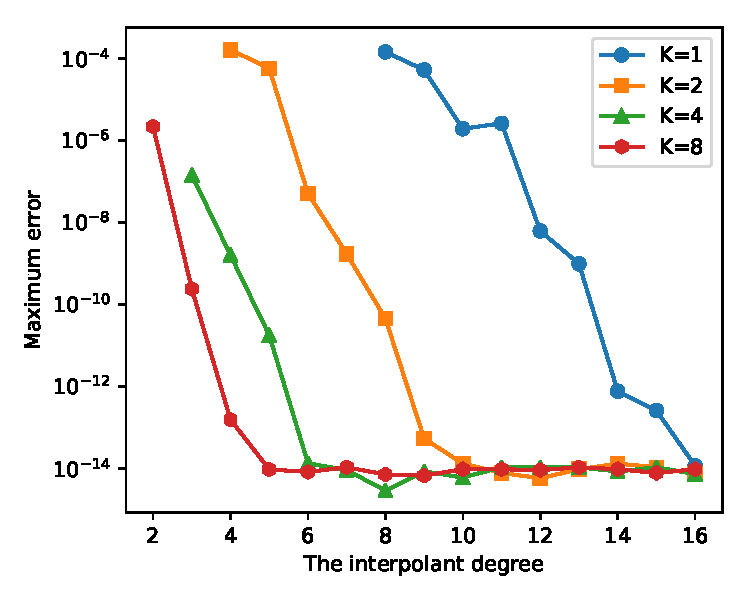
\includegraphics{tex/figures/interpolant_error_after_newton}
	\fautor
	\label{fig:interpolant_error_after_newton}
\end{figure}


\section{An Algorithm for MCER}\label{section:mcer}

This section introduces the elliptical PMCLP where there is no axis-parallel constraint, that is, the ellipses can be freely rotated. We refer to this problem as \sigla{MCER}{Maximal Covering by Ellipses with Rotation}. In comparison with MCE, this problem introduces a new a new variable which is responsible for determining the rotation angle of every ellipse making MCER a more challenging problem.

\section{Definition}

An instance of the non-axis-parallel is defined exactly like the axis-parallel one on \autoref{chapter:ellipses}. It is given by a set of demand points $\Pp=\{p_1, \dots, p_n\}$, $p_j\in\R^2$; a list of weights $\Ww:=\{w_1, \dots, w_n\}$, with $w_j\in\R_{\ge0}$ being the weight of point $p_j$;
and a set of $m$ axis-parallel ellipses given by their shape parameters $\Rr:=\{(a_1, b_1), \dots, (a_m, b_m)\}$, with $(a_j, b_j)\in\R_{>0}^2$ and $a_j>b_j$.
Additionally, to make the text more clear, we define a set of $m$ ellipses as $\E = \{E_1, \dots, E_m\}$, with $E_j : \R^2\times\R^2 \mapsto \R^2$ being a function that takes the center and angle of rotation where the $j$-th ellipse is located as input, and returns its coverage region.

Given an instance of $MCER$, we define $Q:=(q_1, \dots, q_m) \in \R^{2m}$ to be the centers of each ellipse, $\Theta:=(\theta_1, \dots, \theta_m) \in [0, \pi)^m$ to be the angle of rotation of each ellipse and $E_i(q_i, \theta_i)$ to be the coverage region of ellipse $E_i$ with its center at point $q_i$ rotated by angle $\theta_i$, which is given by \autoref{eq:rotated_ellipse_co}. Therefore MCER is defined as the problem of determining $Q$ and $\Theta$ (placing and rotating each ellipse) to maximize the weight of points covered by the $m$ ellipses, which is given by

\begin{equation}\label{eq:optMCEn}
\max_{Q, \Theta}{w\left(\bigcup_{i=1}^{m} \Pp \cap E_i(q_i, \theta_i)\right)}.
\end{equation}

An additional notation is used on this chapter, $\tilde{E_i}(q_i, \theta_i)$ is defined to be the set of points on the border of $E_i(q_i, \theta_i)$, specially, the operation $\Pp \cap \tilde{E_i}(q_i, \theta_i)$ is used to refer to the set of points from $\Pp$ that lie on the border of $E_i(q_i, \theta_i)$.


\begin{proposicao}\label{lema:mce_2b}
	Let $(\Pp, \E)$ be an instance of MCER. In an optimal solution of MCER, for any $E_j \in \E$, such that $|\Pp \cap E_j(q_j, \theta_j)|\ge2$, there is $q_j'$ such that $\Pp \cap E_j(q_j', \theta_j)=\Pp \cap E_j(q_j, \theta_j)$ and $\Pp \cap \tilde{E_j}(q_j', \theta_j) \ge 2$.
\end{proposicao}

\begin{demonstracao}
	First, the angle of rotation can be ignored as it does not change.
	
	Let $A=\Pp \cap E_j(q_j, \theta_j)$ be the set of points covered by $E_j$ and $X=\cap_{p \in A}E_j(p, \theta_j)$ be the region of intersection of ellipses centered at each point from $A$.

	As it was shown on \autoref{chapter:ellipses}, $X$ is a region that is limited by arcs of ellipses. As this region is the non-empty intersection of more than one ellipse, there are at least two of these arcs that encounter at one point creating a vertex. Selecting any of these vertices as $q_j'$ will make $|\Pp \cap \tilde{E}_j(q_j', \theta_j)| \ge 2$.
	
\end{demonstracao}

What \autoref{lema:mce_2b} is saying is that any optimal solution for MCER can be transformed into another optimal solution where every ellipse covers the same set of points and those which cover more than one point has two points on their border. Also, this equivalent optimal solution can be always achieved by just translating the ellipses. An example is shown on \autoref{fig:ellipse-2-points} for one ellipse.

A lot of the ideas developed in this chapter are based on fixing two points on the border of an ellipse, which is why \autoref{def:feasible_angle} introduces a new notation for angles that an ellipse rotated by it can be translated into a center, such that it contains two fixed points. 

\begin{figure}[H]
	\centering
	\caption{An optimal solution before and after applying \autoref{lema:mce_2b}.}
	\includegraphics{tex/figures/scripts/ellipse-2-points}
	\fautor
	\label{fig:ellipse-2-points}
\end{figure}

\begin{definicao}\label{def:feasible_angle}
	Let $E$ be an ellipse and $u, v \in \R^2$. An angle $\theta \in [0, \pi)$ is said to be $(E, u, v)$-feasible if there is $q \in \R^2$ such that $\{u, v\} \subset \tilde{E}(q, \theta)$.
\end{definicao}

On \autoref{fig:feasible-angle} two examples for \autoref{def:feasible_angle} are shown. On one of them, an ellipse is rotated by $\pi/4$ and it is located such that it contains the two fixed points on its border. That means $\pi/4$ is a $(E, u, v)$-feasible angle. On the other example, the ellipse is rotated by $\pi/2$ and there is not a center where the ellipse can be placed so it contains the two fixed points--they are too far apart. This makes $\pi/2$ a not $(E, u, v)$-feasible angle.

\begin{figure}
	\centering
	\caption{A $(E, u, v)$-feasible angle and a not $(E, u, v)$-feasible angle.}
	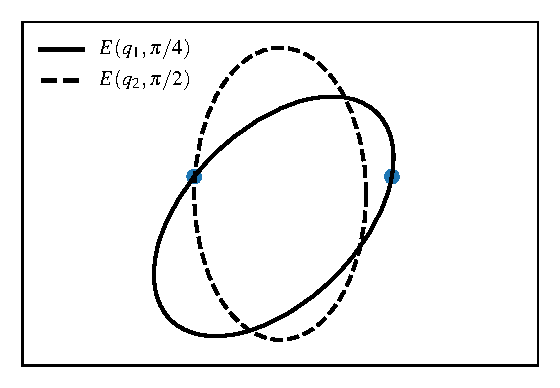
\includegraphics{tex/figures/scripts/feasible-angle}
	\fautor
	\label{fig:feasible-angle}
\end{figure}

\begin{lema}\label{lema:3pnts}
	Let $(\Pp, \E)$ be an instance of MCER, in an optimal solution, for any $E_j \in \E$, such that $|\Pp \cap E_j(q_j, \theta_j)|>2$, at least one of the two cases is true:
	
	\begin{enumerate}
		\item There is $q', \theta'$, and $\{u, v, w\} \subset \Pp \cap E_j(q_j, \theta_j)$, such that $\{u, v, w\} \subset \tilde{E}(q', \theta')$.
		
		\item Let $A=\Pp \cap E_j(q_j, \theta_j)$, and $u, v \in A$ such that there exists $\hat{q}_j$ such that $\{u, v\} \subset \tilde{E_j}(\hat{q}_j, \theta_j)$ and $A \subset E_j(\hat{q}_j, \theta_j)$. Then for any $(E_j, u, v)$-feasible angle $\theta \in [0, 2\pi]$, there exists $\bar{q}_j$ such that $\{u, v\} \subset \tilde{E_j}(\bar{q}_j, \theta)$ and $A \subset E_j(\bar{q}_j, \theta)$.
	\end{enumerate}
\end{lema}

The first case of \autoref{lema:3pnts} is saying that there is another optimal solution which has $E_j$ covering the same set of points, but with three points on its border. 

The second case of \autoref{lema:3pnts} says that after fixing a pair of points on the border of $E_j$ maintaining the covered set, for any angle that allows the two points to stay on the border of $E_j$, there is a center that maintains the covered set the same.

On \autoref{fig:lema-3-points} both cases of \autoref{lema:3pnts} are shown. There, it can be seen that for the second case, it does not matter which feasible angle by which the ellipse is rotated, the third point will always be inside the coverage area. Also, an example of the first case is shown where there are three points lie exactly on the border of the ellipse.

\begin{figure}
	\centering
	\caption{An example of \autoref{lema:3pnts}.}
	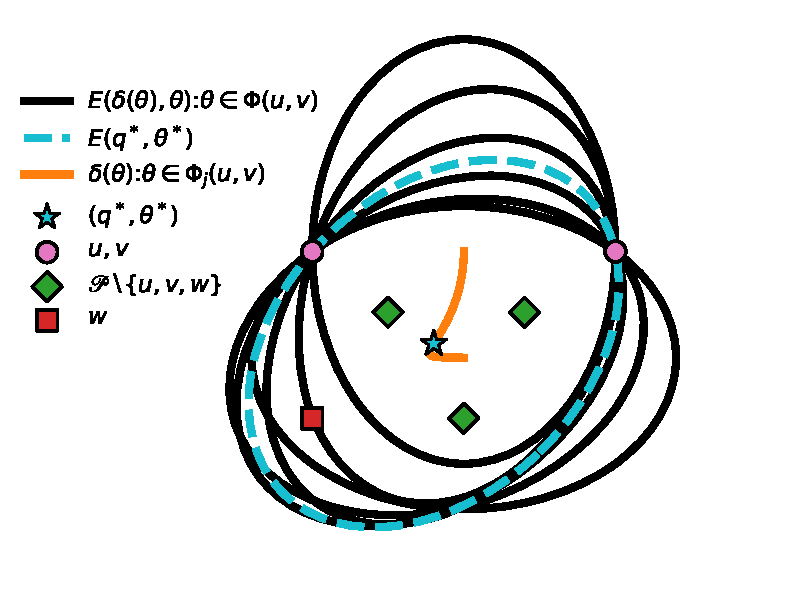
\includegraphics{tex/figures/scripts/lema-3-points}
	\fautor
	\label{fig:lema-3-points}
\end{figure}

The idea to prove \autoref{lema:3pnts} is that after fixing $u, v$ on the border of $E_j$, which is possible by \autoref{lema:mce_2b}, the movement of rotation and translation while keeping $u, v$ on the border is continuous. Because of that, the negation of case two implies case one and vice versa.


If we define an equivalence relation between optimal solutions as: $S_1$ is equivalent to $S_2$ if they both cover the same set of points, we can use \autoref{lema:3pnts} and \autoref{lema:mce_2b} to identify the equivalence classes. Let $S$ be any optimal solution, in $[S]$ (its equivalence class) there is another solution where any ellipse $E_j \in \E$ falls in at least one of the cases below:
\begin{itemize}
	\item $E_j$ covers only one point.
	\item $E_j$ covers more than one point with $u$ and $v$ being on the border of $E_j$. Note that there could be infinitely many of solutions like that, however, \autoref{lema:3pnts} guarantees that any $(E_j, u, v)$-feasible angle yields an equivalent optimal solution.
	\item $E_j$ covers more than two points with three of them on its border.
\end{itemize}

The following two sections will treat the second and third cases (the first case is trivial). Going through every possibility of an ellipse falling in any of the three cases guarantees that an optimal solution is found.

\section{Ellipse by two points}

Let $E$ be an ellipse with shape parameters $(a, b)\in \R^2_{>0}$ and $u, v\in \R^2$, one wants to find a $(E, u, v)$-feasible angle $\theta\in[0,\pi]$ and every center $q\in\R^2$ such that $\{u, v\} \subset \tilde{E}(q, \theta)$.

For a fixed angle, finding every center such that two points are on the border of the ellipse is done on \autoref{chapter:ellipses_intersection}, from there we know that there could be at most $2$ of such centers. The only thing left to be done is finding a feasible angle. It turns out that the angle that makes the major-axis of the ellipse to be aligned with the line that passes through $u$ and $v$ will be a feasible angle if, and only if the set of feasible angles is not empty. This can be seen geometrically as other angles achieve a lesser maximum distance between the two points on the border.

\section{Ellipse by three points}




\section{Reducing the CLS size}\label{section:reducing_cls}
As for the algorithms for both MCE and MCER, the number of solutions they go through is directly proportional to the size of each ellipse's CLS, reducing their size can significantly improve the performance of both algorithms. 

For MCE (the MCER's case is analogous), let $q, q' \in S_j$ be two possible locations in the CLS for the $j$-th ellipse. If $\Pp \cap E_j(q') \subset \Pp \cap E_j(q)$, then $q'$ is redundant and we can remove it from $S_j$, as it produces a solution which is either non-optimal or equivalent to an optimal one.

To remove redundant elements from a CLS, we use the same tree-like data structure described in \cite{andreta}, which keeps every maximal subset of covered points by an ellipse, and supports a query operation to verify if a subset is maximal or not.
First, we sort the elements in $S_j$ by the number of covered demand points, non-decreasingly. Then, we iterate over it, removing elements which make the ellipse cover non-maximal subsets of demand points, when compared to the elements of $S_j$ that have already been processed.


\section{Prunning the Backtracking Tree}\label{section:prunning}
In this section, we introduce a condition for skipping solutions in the backtracking process in the algorithms for MCE and MCER.
The idea is to prune the backtracking tree by observing that any solution constructed going down the current branch will have a value less than or equal to the current best solution.
As this condition can be applied for both problems, and their notation differs very little, we describe it only for MCE.

Given an instance $(\Pp, \Ww, \Rr)$ of MCE, an upper-bound for the value of an optimal solution is the sum of the optimal solutions for each ellipse individually:
\begin{equation}\label{eq:upper-1}
\max_{Q} w\left(\bigcup_{j=1}^m \Pp \cap E_j(q_j)\right) \le \sum_{j=1}^m \max_{q_j} w(\Pp \cap E_j(q_j)).
\end{equation}

Suppose that the first $k$ ellipses are fixed at locations $(q_1,\dots, q_k)$, and that we have a lower-bound $L$ for the value of an optimal solution. Let $Z_k=\Pp\setminus \cup_{j=1}^k E_j(q_j)$ be the points not covered by the first $k$ ellipses, then we can use \autoref{eq:upper-1} to verify if we can skip every solution where the first $k$ ellipses are fixed at  $(q_1,\dots, q_k)$ or not.
If
\begin{equation}\label{eq:upper}
w\left(\bigcup_{j=1}^{k} \Pp \cap E_j(q_j)\right)+
\sum_{j=k+1}^m \max_{q_j} w(Z_j \cap E_j(q_j)) \le L,
\end{equation}
then, any solution with the first $k$ ellipses fixed at $(q_1,\dots, q_k)$ will have value less than or equal to the value of an optimal solution, therefore, we can cut the backtracking tree there. In practice, we can use the value of the best solution found at the moment as the lower-bound $L$.

It is worth mentioning that this improvement do not have an effect in a possible worst case scenario. We decided to adopt it in our implementation because it showed good results in practice.
For example, without it, 
MCER-$k$'s algorithm takes nine seconds to obtain an optimal solution for instance AB060 developed by \cite{andreta}, going through \num{336494451} solutions, while the implementation using \autoref{eq:upper} to prune the backtracking tree for the same instance takes less than one second to return an optimal solution, and evaluates only \num{1809} solutions in total.


\section{Numerical Experiments}\label{section:numerical}

\section*{References}
	%% New version of the num-names style
	\bibliographystyle{elsarticle-num}
	\bibliography{../references}
	
\end{document}

%%
%% End of file `elsarticle-template-1-num.tex'.